
\chapter{Implementation and Results}

\section{Simulation}\label{section:Implementation}
Simulation using path generation, path following control and EKF combined.

\section{Hardware}\label{section:Hardware}
Verify EKF using Hardware
Description of the Hardware
Pixhawk 2.1 CubeBlack, Intel Edison, APSync, Ardupilot ArduCopter 4.1. 
Sensors onboard the Cube, plus OFS and GPS external sensors.

In addition to the simulation results, test flights were conducted with a custom hexacopter with the aim of collecting data to verify the EKF algorithm.

\begin{figure}[htb]
	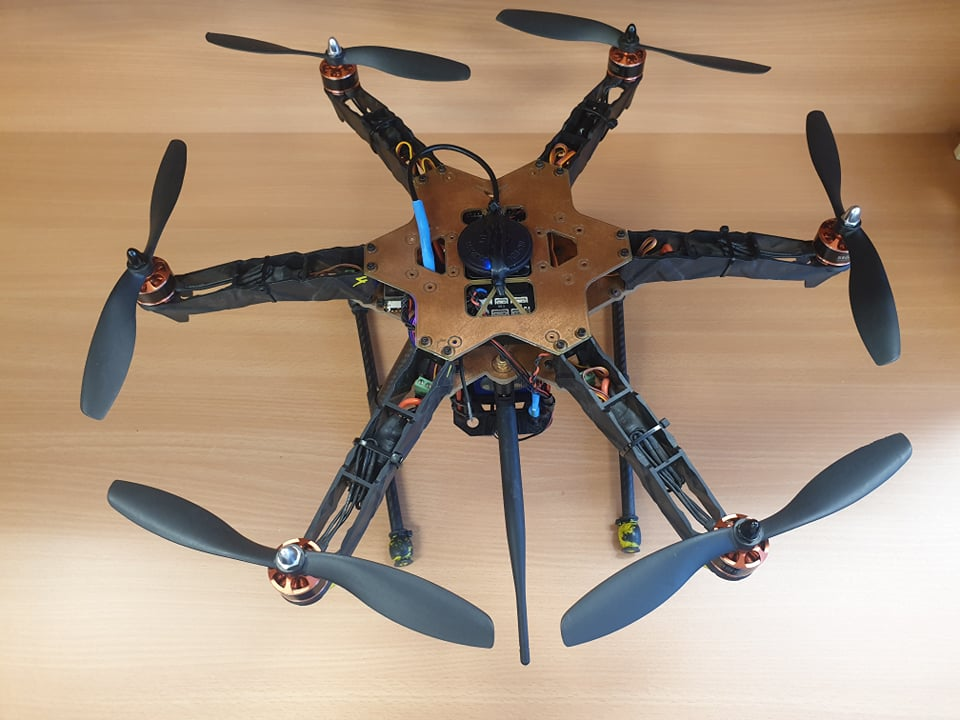
\includegraphics[width=\columnwidth]{Hexacopter_Hardware.jpg}%
	\caption{Hardware platform used for flight testing.}%
	\label{fig:hardware}%
\end{figure}

\subsection{The Cube Autopilot}
The drone is controlled by a commercial flight controller known as The Cube Autopilot (formerly known as Pixhawk 2.1).
\subsection{ArduPilot Software}
The vehicle is controlled using the open source flight software Ardupilot, with the specific version being ArduCopter 4.1.
\subsection{Companion Computer}
Additionally, a computer-on-module known as the Intel Edison was added to the Cube flight controller in order to enhance the system capabilities and enable wireless communication. The Edison has a 500 MHz dual-core processor, 1 GB RAM, 4 GB storage and dual-band (2.4 and 5 GHz) WiFi connectivity.

APSync, an open source software package developed for use with ArduPilot, was installed on the Edison. This included a Linux operating system as well as a number of python and DroneKit packages. DroneKit is an open source API which allows python scripts to be run on flight control hardware. The relationship between the different systems is shown in figure .......

\subsection{Sensors}
The Cube flight controller contains three sets of IMUs (accelerometer, gyroscope and magnetometer), two of which are mechanically vibration-isolated. Two of the IMUs are the Invensense MPU9250 and the third is made up of the STM LSM303D (accelerometer and magnetometer) and L3GD20 (gyroscope). The Cube also contains two barometers, both of which are the MS5611. Multiple of each kind of sensor are provided for redundancy and the EKF in the ArduPilot firmware fuses the data from all sensors for additional accuracy.

Additional sensors were connected to the Cube Autopilot system to enable the previously developed EKFs to be tested.  

A GPS module, Ublox NEO-M8N, was connected to the Cube. This module also housed a magnetometer for additional external measurement of the Earth's magnetic field. The GPS module communicates with the flight controller via the I2C protocol.


An integrated optical flow and lidar sensor, Matek 3901-L0X, was also connected to the system. This module consists of a Pimoroni PMW3901 optical flow sensor, an Adafruit VL53L0X lidar sensor and a STM32L051 microcontroller, as well as additional power regulating circuitry. This sensor is able to communicate over UART using Multiwii Serial Protocol (MSP), which is supported by the ArduPilot firmware.

\subsection{Flight Testing}
Flight testing was conducted by programming the hexacopter with an autonomous mission, which involved taking off to a height of 1.5 metres, travelling approximately 11 metres to a second position and landing. The drone performed the mission successfully using the ArduPilot flight control software and the sensor data recorded during the flight was logged to the onboard SD card. This data was processed in MATLAB and used with the EKF algorithm described in Section \ref{section:GPS_EKF}. \figref{fig:HW_GPS_Pos} shows the position and velocity results, and \figref{fig:HW_GPS_Ang} show the angular results. The estimates produced by the previously developed algorithm are compared with the estimates of the ArduPilot (AP) software. Note that for the yaw angle results, an angle of $2\pi$ radians is equivalent to 0 radians, which explains the sudden decline in these results. The estimated yaw angle climbs above $2\pi$ radians before correcting and returning towards zero in the correct range. 

\begin{figure}[htb]
	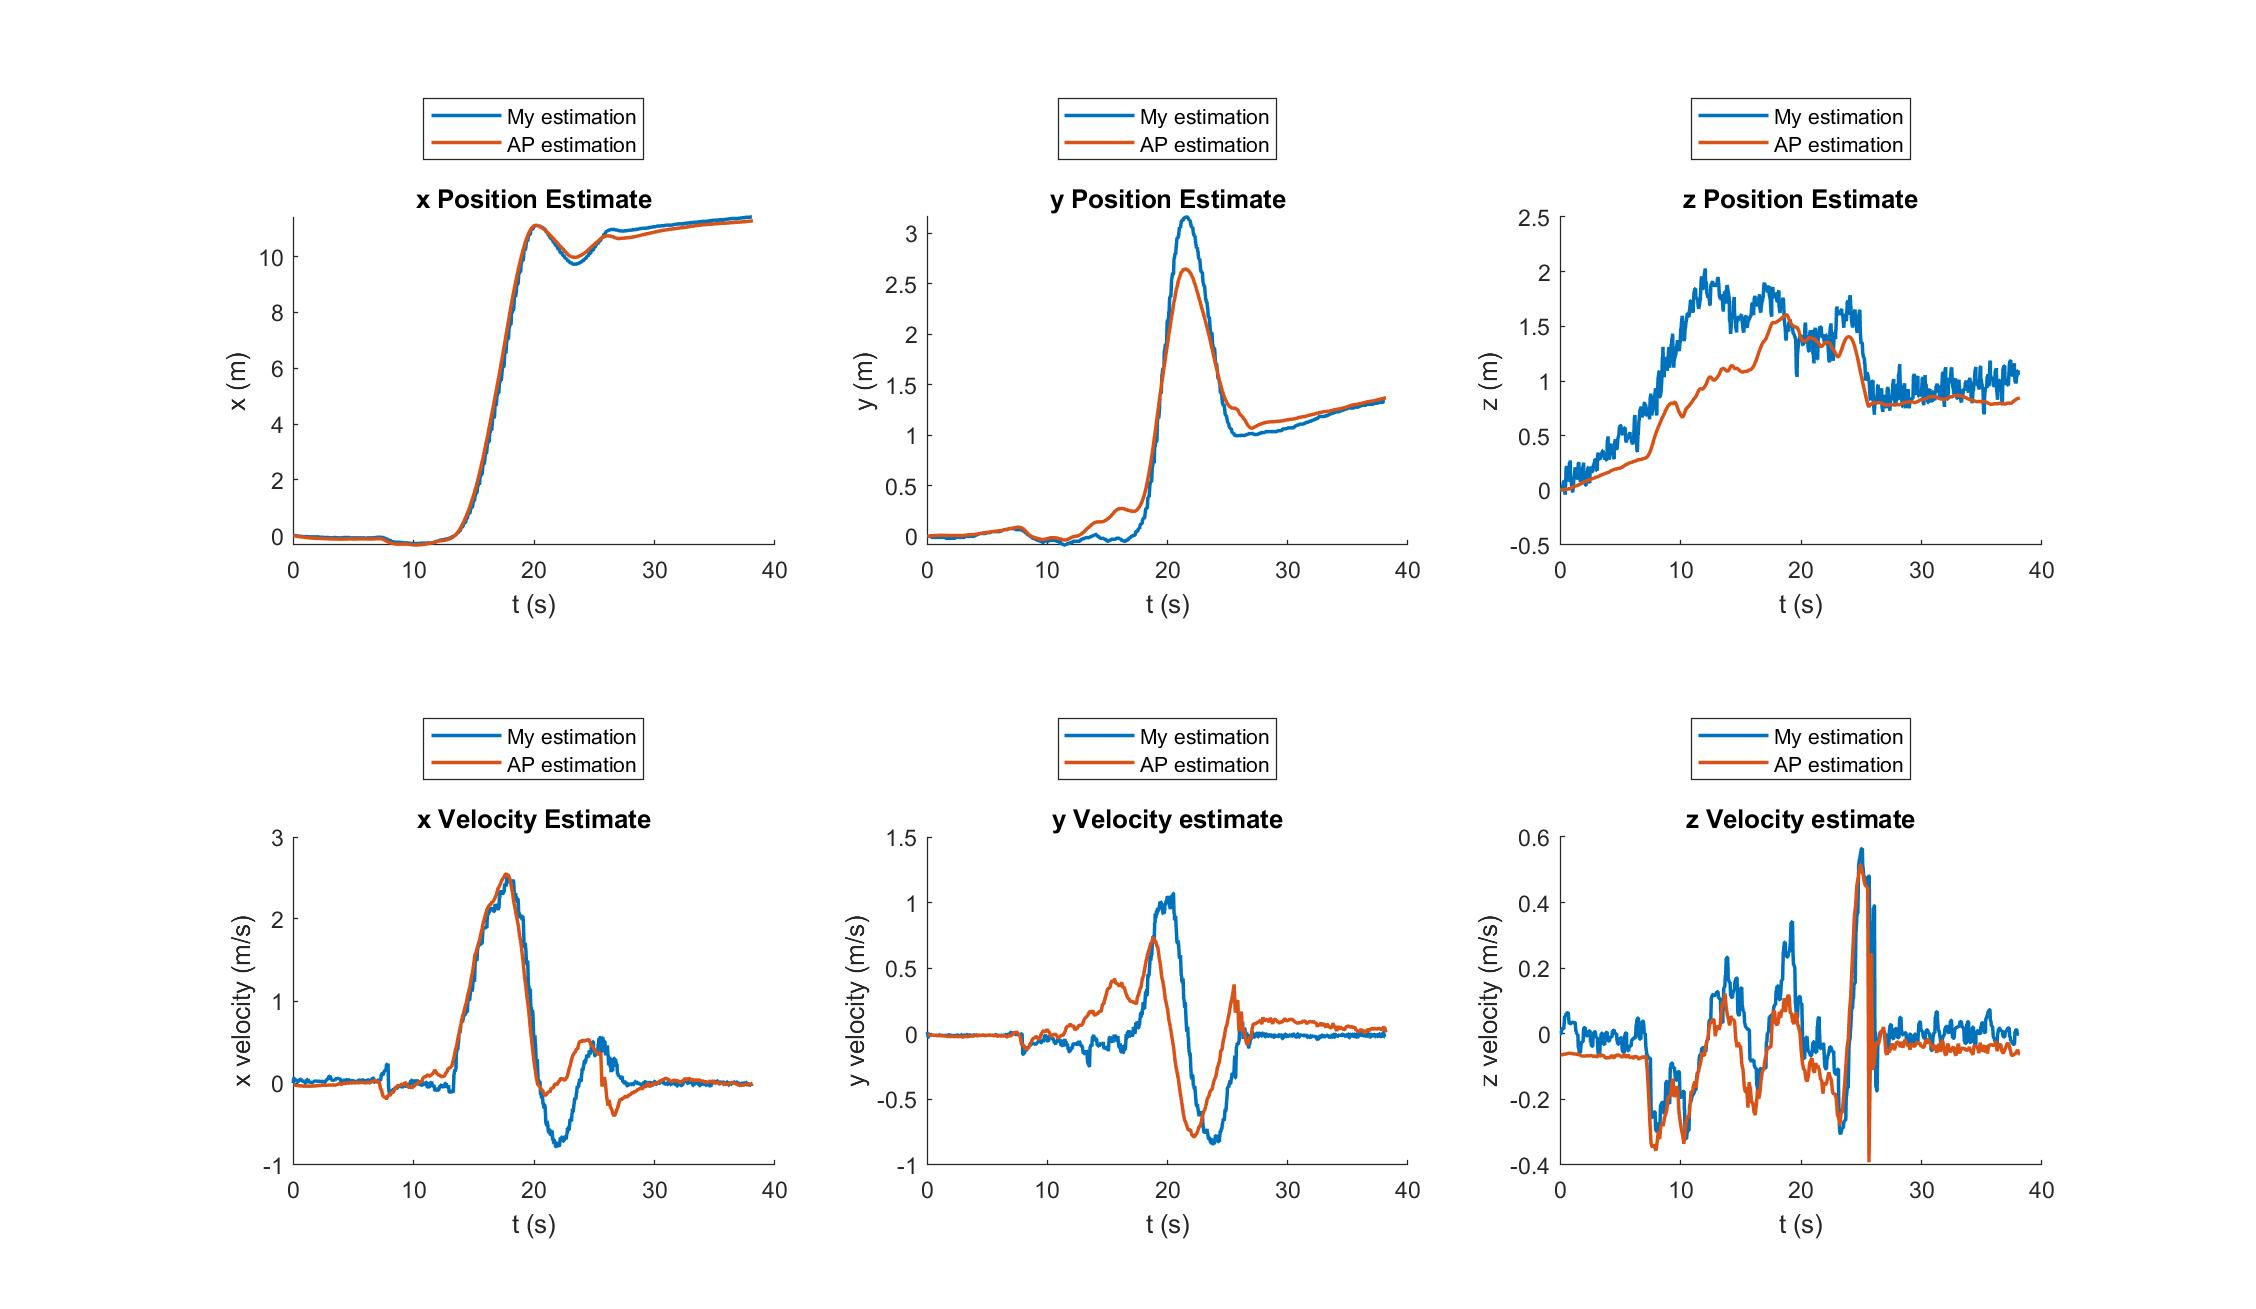
\includegraphics[width=\columnwidth]{EKF_HW/GPS/FlightTest1_Pos.jpg}%
	\caption{The EKF position and velocity estimates compared with the ArduPilot EKF estimates for flight test \#1.}%
	\label{fig:HW_GPS_Pos}%
\end{figure}

\begin{figure}[htb]
	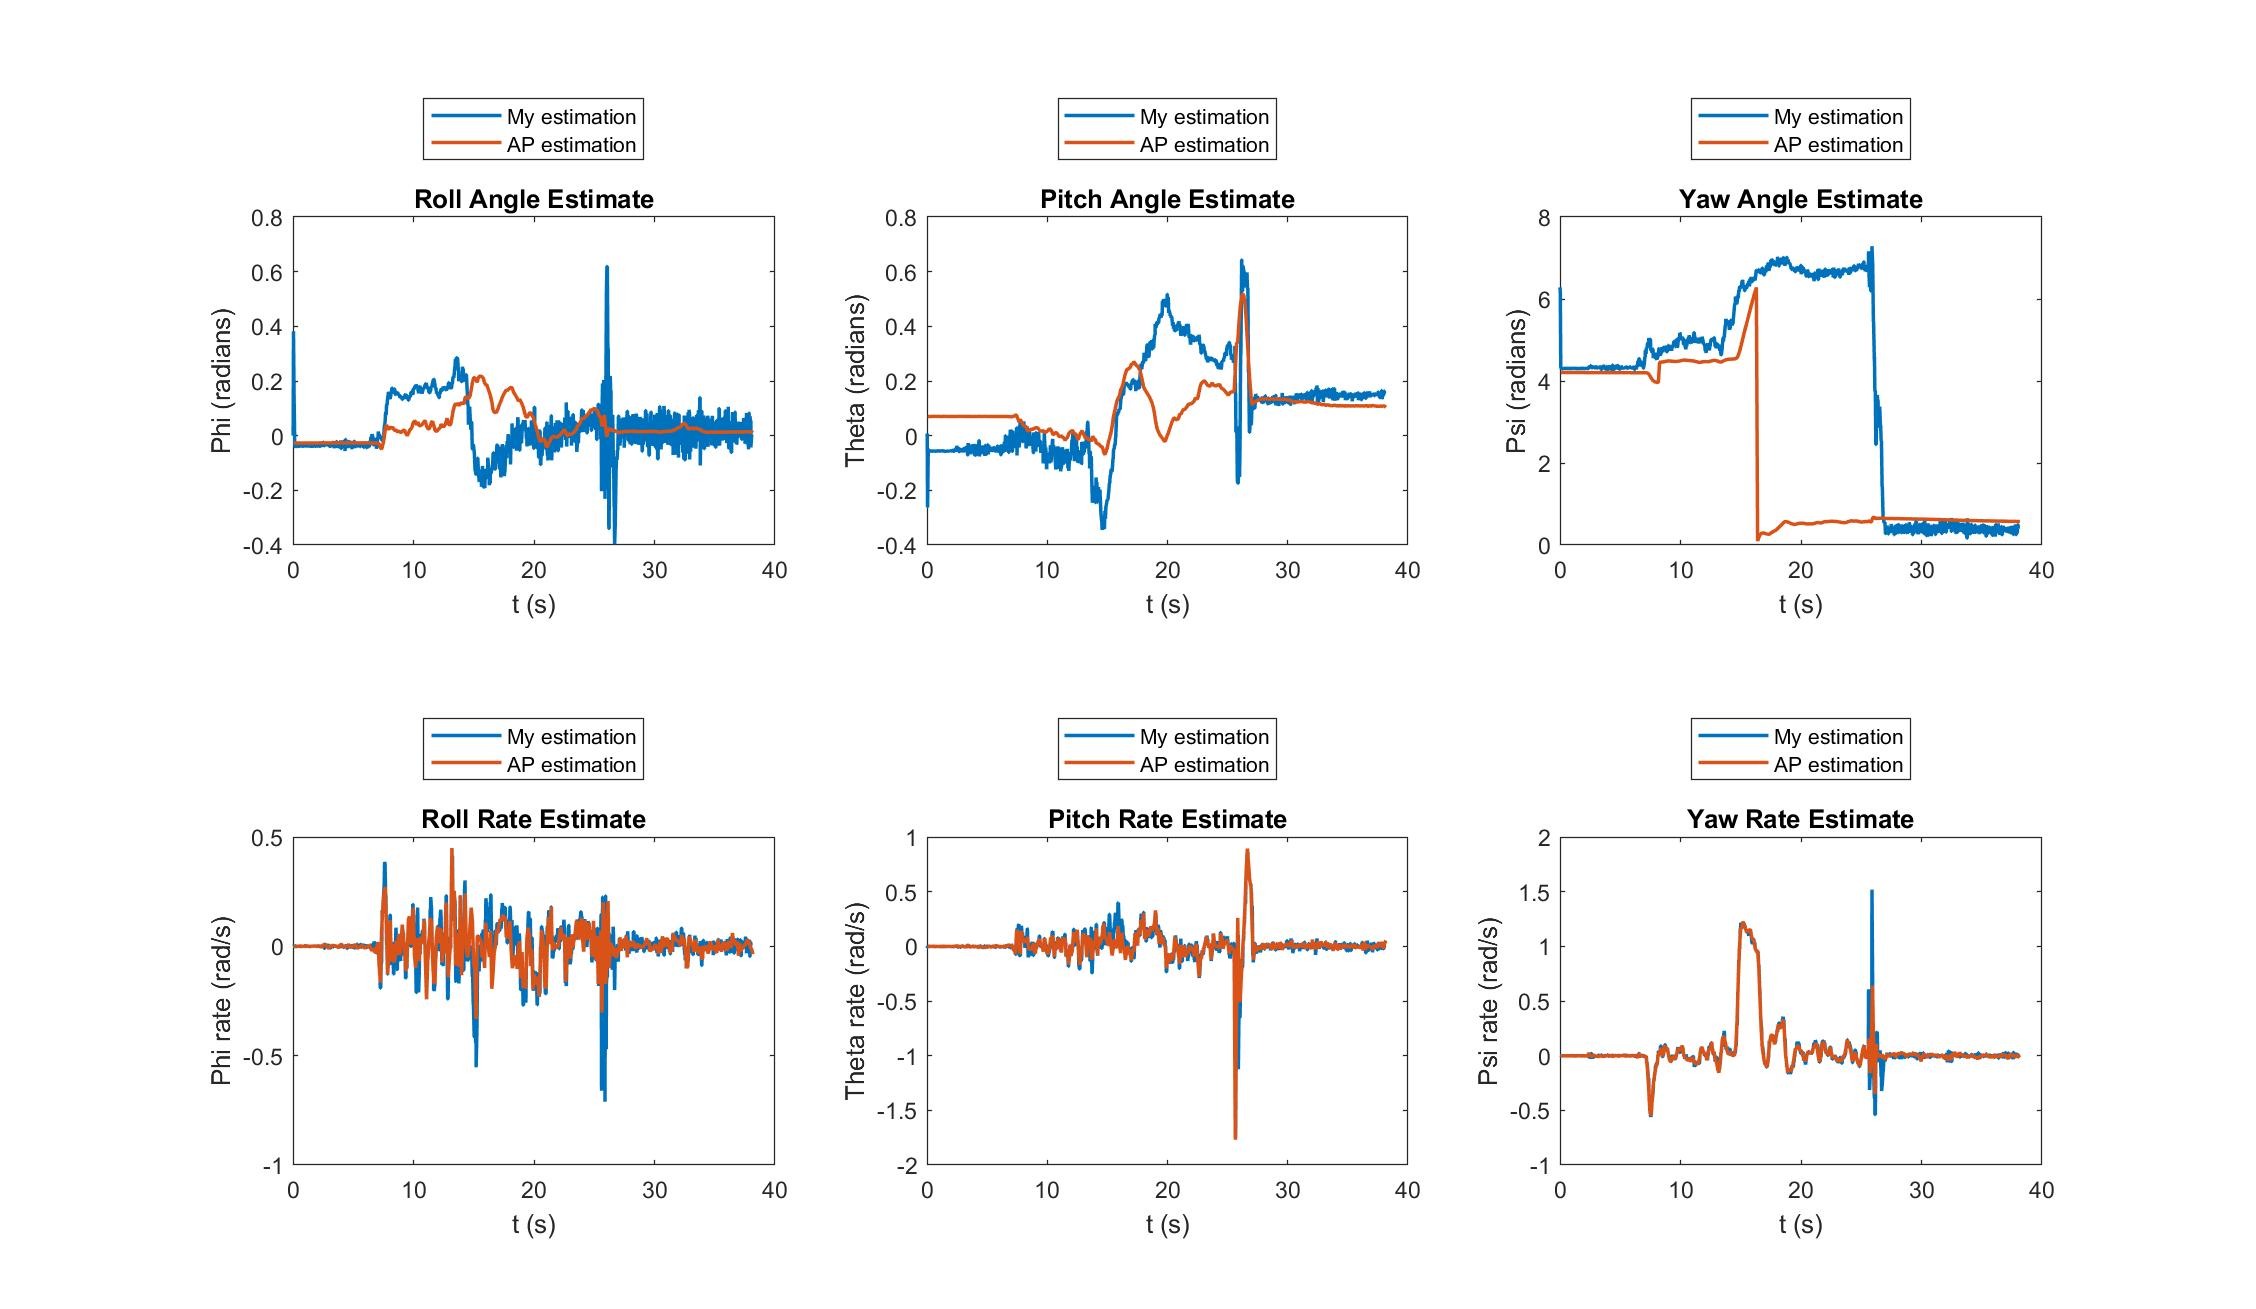
\includegraphics[width=\columnwidth]{EKF_HW/GPS/FlightTest1_Angle.jpg}%
	\caption{The EKF angular estimates compared with the ArduPilot EKF estimates for flight test \#1.}%
	\label{fig:HW_GPS_Ang}%
\end{figure}

A flight test was then repeated with the optical flow sensor installed, in order to evaluate the effectiveness of the EKF in the absence of GPS data. This flight involved taking off to a height off approximately 1.5 m, hovering at that point for approximately 10 seconds and then landing at the same point. The results of the EKF are shown in \figref{fig:HW_OFS_Pos}, compared with the AP estimation (which uses GPS data). The position and velocity estimates are not extremely accurate, however it can be seen that there is no significant drift in the position estimates over this time period.

\begin{figure}[htb]
	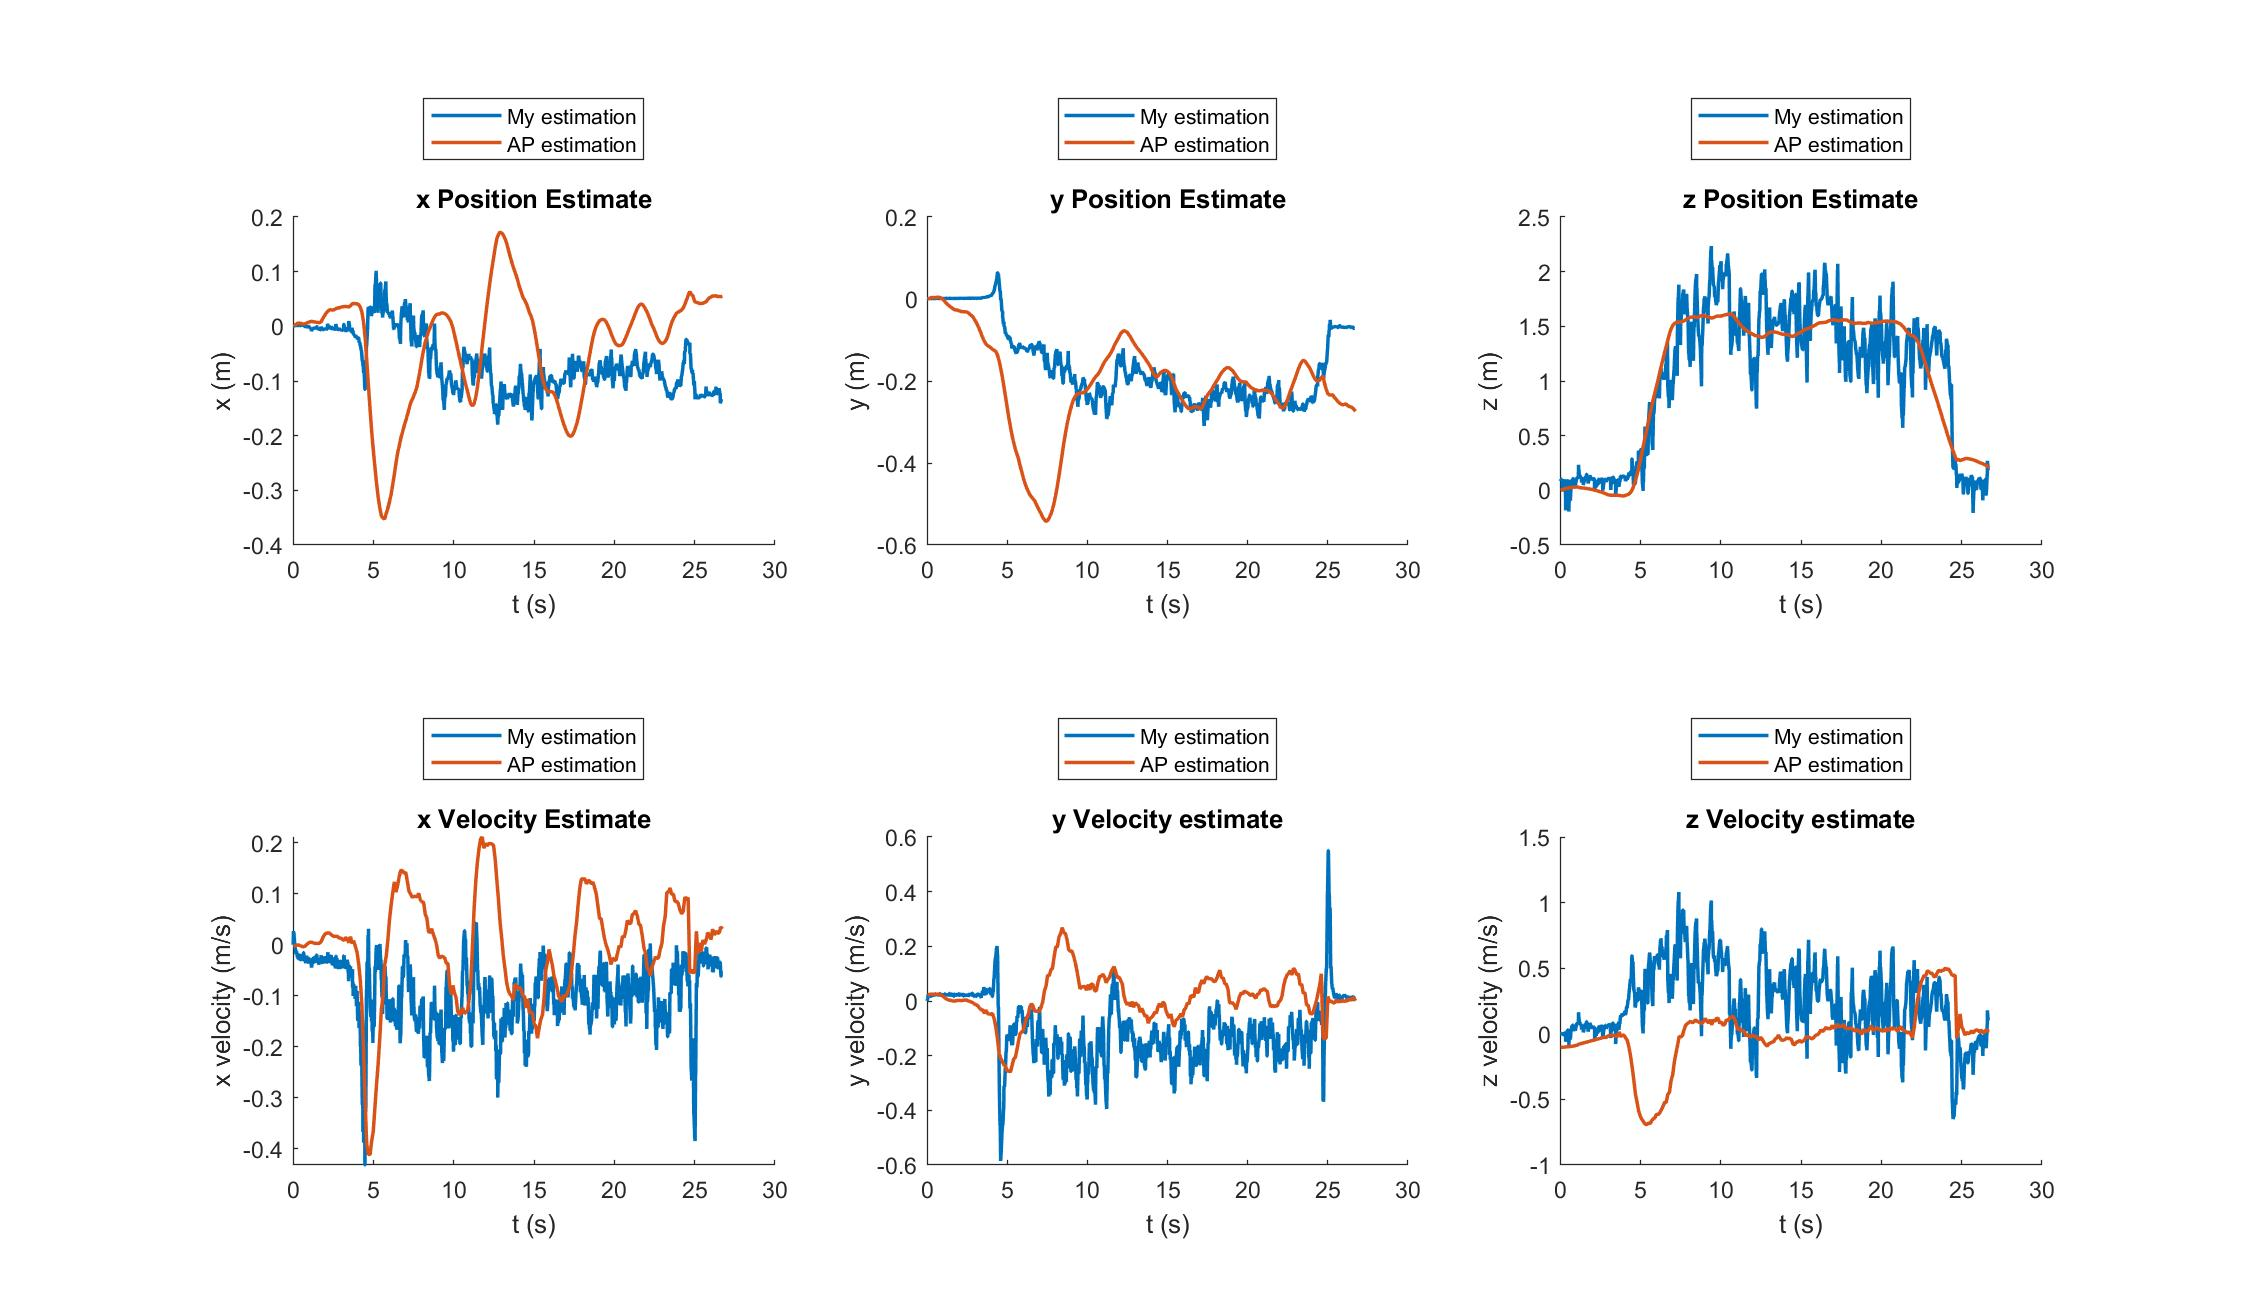
\includegraphics[width=\columnwidth]{EKF_HW/OFS/FlightTest2_Pos.jpg}%
	\caption{The OFS EKF position and velocity estimates compared with the ArduPilot EKF estimates for flight test \#2.}%
	\label{fig:HW_OFS_Pos}%
\end{figure}

A third flight was undertaken in which the aircraft was programmed to take off to 1.5m, hover in place for 10 seconds, then travel some distance to land at another waypoint. This flight resulted in a collision with the ground, however the first 25 seconds of data was able to be used for analysis. Using this data, it could be seen that using the OFS data alone was insufficient for tracking positional change. This is likely due to the slow sampling rate (10 Hz) of this particular sensor and the unreliability of the lidar data.




\FloatBarrier
\section{Chapter Summary}

\clearpage


